\section{Data Collection}
\label{ch:measurement}
The voice comparison raises three measurement questions: whether participants perceived the self-similar voice as resembling their own, whether voice condition changed search performance, and how participants experienced the assistance. Answering them requires outcome measures and a record of the speech each participant actually heard. This section links voice identity, delivered speech, search events, and questionnaire responses. Perceived similarity is reported as a manipulation check, kept distinct from performance and experience outcomes. Detailed gaze and timing records support the interpretation of these outcomes, and Appendix~\ref{app:instruments} gives instrument wording and scoring.


\subsection{Frame-Level Records and the Trial CSV}
Follow My Voice records time-varying observations separately from trial summaries. Each frame record stores application time, gaze origin and direction with tracking validity, head pose, available controller poses and input state, and the gaze/controller object-intersection evidence used by guidance. Object identities and transforms provide the scene needed for reconstruction. Guidance transitions, agent decisions, actual speech playback, trigger selections, and pauses are recorded as events. A rendered frame can reuse a sensor observation, so frame counts differ from the number of independent eye-tracking samples.

The trial replay snapshot stores the wall bottom in recording-local coordinates, the wall height in metres, and a flag indicating that these bounds are available. Trial Review uses these values to reconstruct the walls. Earlier recordings lack the bounds, so their walls are reconstructed from object-derived wall estimates and the original object positions, without rescaling to the current layout. The replay fields supplement the saved layout version and transforms and are separate from the trial CSV columns. Wall geometry differs between the two layouts, so analyses that combine recordings from both retain the layout version.

Trial Review generates an Excel-compatible trial CSV with one row per trial. Its fields describe task performance, geometry, guidance exposure, and associated subjective responses (Table~\ref{tab:trial-fields}). Outcome, practice, provenance, and quality information accompany the exported records to support analysis and eligibility checks.

\begin{table}[htbp]\centering
\caption[Trial CSV contents]{Contents of the trial CSV. Unavailable values and reserved, uncollected fields are left blank.}
\label{tab:trial-fields}
\small\tagpdfsetup{table/header-rows={1}}
\begin{tabularx}{\linewidth}{@{}p{0.23\linewidth}X@{}}\toprule
Group & Recorded or derived columns \\\midrule
Identity & Participant ID, trial ID, block index, voice condition. \\
Geometry & Absolute and signed nominal theta; actual signed head-to-target yaw; target-minus-head height; target distance. \\
Guidance and duration & Instruction count and search exposure in seconds. \\
Target contact & Time to first and final target gaze contact; first right-controller target contact; final selection. \\
Subjective context & NASA-TLX score; reserved subjective performance rating, left blank pending an instrument mapping. \\\bottomrule
\end{tabularx}
\end{table}

The yaw and height in the export are head-relative and measured after onset. The pre-cue, cross-relative geometry is stored in the trial summaries and event log. Gaze-contact times are ray intersections, not validated fixations. A questionnaire score repeated across trial rows remains a single block-level observation.

\subsection{From Interaction Events to Research Variables}
The recorded data serve two purposes: reconstructing what happened in a trial and estimating the study outcomes. Reconstruction requires observations and events at their original temporal resolution, whereas statistical analysis usually requires a more compact table. Trial summaries are therefore stored separately from gaze, head/controller motion, object layouts, and event streams. Each summary is a derived representation of the underlying evidence, not a replacement for it.

Each derived value has an identifiable source and definition. For example, a number called ``time to gaze'' is ambiguous unless it specifies the clock origin, the contact rule, validity handling, and the treatment of missing observations. The recorded data keep these distinctions in separate fields.

Figure~\ref{fig:data-provenance} shows how a trial CSV stays linked to the underlying observations. Values prepared for statistical analysis can therefore be traced back to the records needed for trial reconstruction.

\begin{figure}[htbp]
\centering
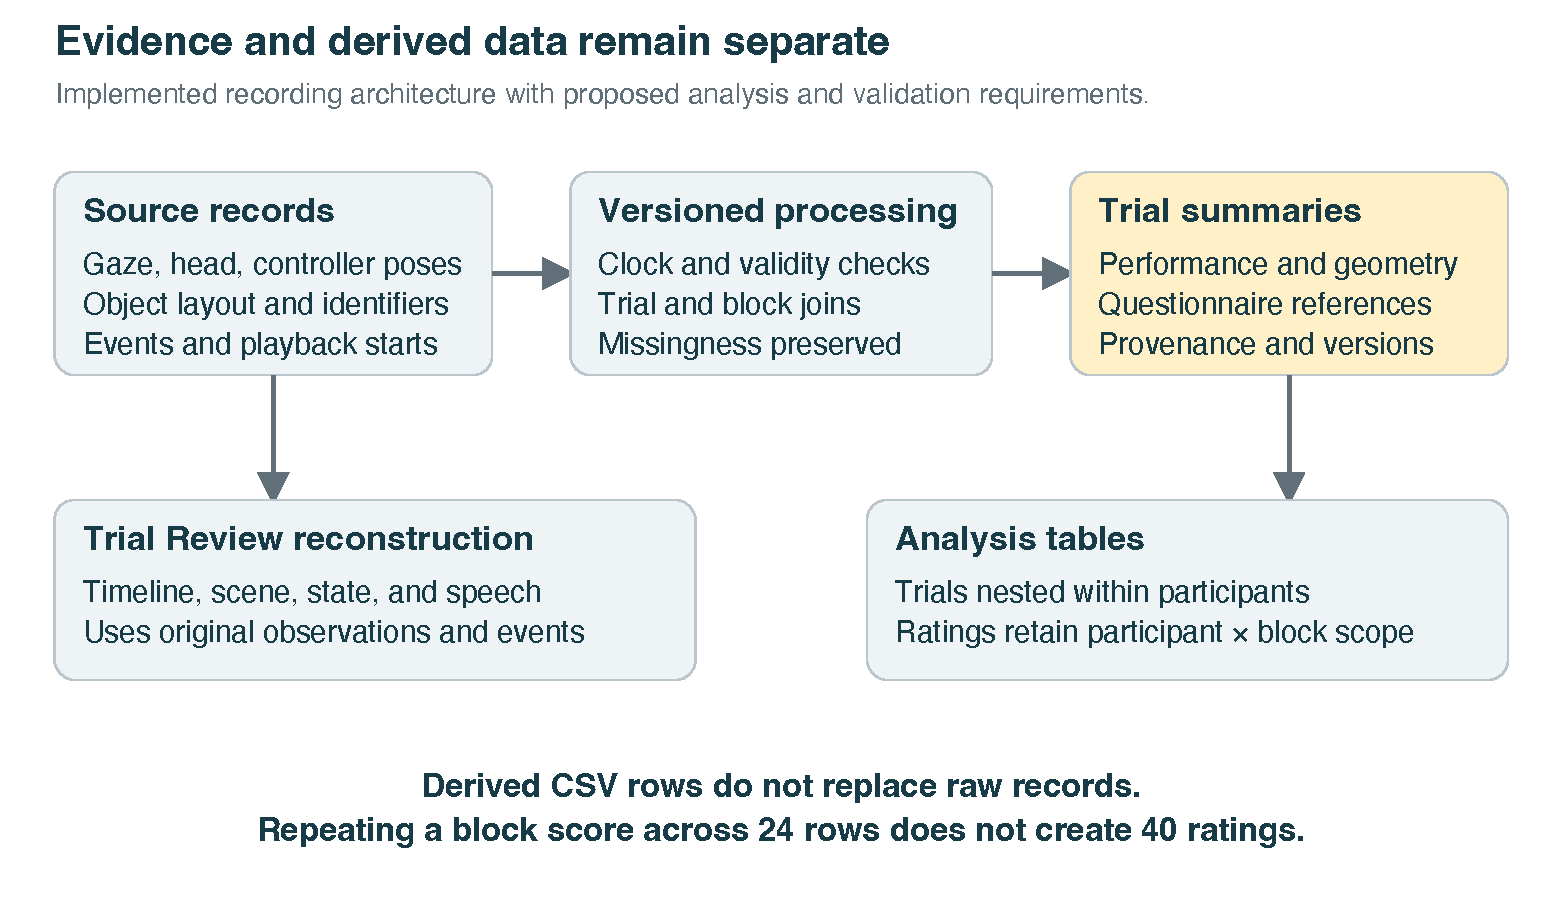
\includegraphics[width=\linewidth,alt={Raw observations and events feed versioned processing, trial summaries, Trial Review, and analysis tables.}]{figures/data-provenance.pdf}
\caption[Raw records, derived summaries, and analytical scope]{Recording and processing relationships. Source streams support reconstruction; derived summaries support analysis. Processing and scoring follow versioned definitions. Block-level ratings repeated in trial rows remain single block-level observations.}
\label{fig:data-provenance}
\end{figure}


\subsection{Geometry, Timing, and Data Quality}
Several measurement definitions are specified in detail in Appendix~\ref{app:measurement-definitions}. The starting angle $\theta_0$ is the signed horizontal angle between the readiness cross and the target, computed from a snapshot saved when readiness completes, and target height is measured relative to the cross (Section~\ref{sec:starting-geometry}). Active completion time runs from object reveal to correct selection and excludes the union of recorded pause intervals (Section~\ref{sec:trial-clocks}). The effective eye-tracking acquisition rate is estimated from distinct source observations rather than rendered frames and is reported with validity, gaps, and spatial-validation error (Section~\ref{sec:acquisition-rate}). Software delivery latency runs from the qualifying event to the actual software playback start of the corresponding cue (Section~\ref{sec:sequence-latency}). Questionnaire responses are joined to blocks through the saved condition order and keep their scale metadata (Section~\ref{sec:questionnaire-joins}).

\subsection{Missed Targets}
A missed target is a search that reaches its recorded 25-second active-search deadline without a correct trigger selection. An incorrect selection followed by a correct selection before expiry is a completed search, with its selection error retained separately. Technical stops, withdrawal, and recordings without a known terminal outcome are not automatically classified as misses. For each participant, block, voice condition, and recorded deadline, the descriptive missed-target percentage is
\begin{equation}
M=100\frac{N_{\mathrm{timeout}}}{N_{\mathrm{selected}}+N_{\mathrm{timeout}}}.
\end{equation}
The denominator excludes practice and unresolved or technically interrupted attempts, and their counts are reported alongside the percentage. A zero denominator yields an unavailable percentage. In the full trial export, \texttt{missed\_target} is 1 for timeout, 0 for successful completion, and blank otherwise. A separate \texttt{missed\_targets.csv} records grouped counts, deadlines, and development-data exclusion labels. Legacy records without an explicit deadline are retained but excluded from this deadline-specific percentage.

This outcome follows Chiossi et al.'s distinction between successful search and searches ending without selection~\cite{chiossi2024searching}. Their task used a five-second limit, whereas the present task is verbally guided with a 25-second limit. Percentages are therefore interpreted within each protocol rather than compared as benchmarks. The six unfinished searches in the earlier development recordings are reported as unfinished rather than as missed targets.

\subsection{Eye-Event and Pupil Measures}
Fixations, saccades, and pupil activity are exploratory measures in this thesis. An offline analysis preserves per-eye directions and pupil diameters from the HTC query stream, deduplicates repeated query timestamps, and separates search from readiness and pauses. Query receipt times record when software obtained the data. Sensor capture time and the independence of consecutive observations remain unestablished. Changes in trial or device, invalid tracking, reversed timestamps, and query gaps longer than 25 ms break continuity. Invalid per-eye observations and observed eye closure exclude nearby 200-ms intervals.

The fixation detector uses elapsed-time dispersion: the sum of horizontal and vertical angular ranges must remain within 1.8 degrees for at least 83 ms. This starting configuration follows the I-DT parameters reported by Chiossi et al.~\cite{chiossi2024searching}, within the detector family described by Salvucci and Goldberg~\cite{salvucci2000fixations}. Azimuth is unwrapped across the signed-angle boundary. The implementation retains event intervals and the duration of eligible segments. Its counts are candidate classifications, not validated fixations.

The saccade detector operates separately, applying a velocity threshold to eye-in-head angular velocity~\cite{salvucci2000fixations}. It uses a provisional 60-degree-per-second threshold, a duration of 20--100 ms, at least two sampled intervals, and observed lower-velocity samples on either side. Intervals with head speed above 20 degrees per second or unavailable head pose are excluded. The reported rate divides event count by retained low-head-speed duration. The rate therefore describes saccades within this restricted window rather than across the whole search. These restrictions reduce head-turn ambiguity, but event identity and sensor-level eye--head synchronization remain unvalidated.

The Index of Pupillary Activity (IPA) calculation follows the wavelet-based approach of Duchowski et al.~\cite{duchowski2018ipa}. Each eye is processed separately. Accepted pupil segments contain valid finite diameters, last at least two seconds, meet a median query-rate screen of 60 Hz, and pass an interval-regularity screen. Within each accepted segment, values are resampled at its median query interval; no interpolation crosses rejected gaps or invalid observations. Level-two sym16 wavelet detail coefficients yield thresholded modulus maxima, which are counted per retained second. The implementation records its thresholds, resampling, numerical tolerance, and nearest-neighbor boundary convention. When no segment qualifies, IPA is recorded as unavailable rather than zero.

Software tests verify event boundaries, query deduplication, invalid-data handling, head-turn suppression, and wavelet calculations. These tests establish computational correctness, not physiological validity. Fixation counts and saccade rates will enter the participant analysis only after independent event annotation, calibration checks, timing assessment, and held-out threshold evaluation in the eye validation session (Section~\ref{sec:measure-validation}). Pupil-based interpretation also requires checks for luminance, gaze angle, blink artifacts, segment boundaries, and task-related confounds. IPA is therefore an exploratory measure reported alongside NASA-TLX, not a validated workload estimate for this apparatus. Final fixation duration on the target remains unavailable until validated eye events can be joined to target areas of interest. The last ray contact does not measure it.

\subsection{Gaze Contact, Vicinity, Pointing, and Selection}
Four event families are central to interpretation: a valid eye ray can intersect the target collider; a gaze direction can satisfy the larger target-vicinity rule; the right-controller ray can intersect the target; and a trigger press can select the target. These events can occur at different times and need not occur in that order in every recorded sample sequence.

The first gaze-contact latency uses the first valid recorded target-ray intersection after reveal. The last gaze-contact time uses the last such intersection before trial end. Neither is a fixation duration. If no contact is observed because of a blink, acquisition gap, or a path that only enters the broader vicinity, the contact field remains missing.

Vicinity qualification is an interaction rule rather than a fixation classifier. In the current system, a target can be acknowledged after 100 ms of valid qualifying evidence, with overlapping regions resolved to a single closest candidate. The rule trades exact collider intersection for a tolerance intended to make feedback usable. An overly large region, however, can produce premature acknowledgment even when the timing gate behaves correctly. The tolerance value will therefore be logged and set through piloting. The default ring in the synthetic viewer screenshot is illustrative, not a validated study setting.

Controller pointing is a distinct input observation, but its spoken acknowledgment also depends on gaze. The acknowledgment requires a qualified one-second controller hold with valid gaze in the target vicinity, and it plays when the speech scheduler permits. Before the hold completes, a valid controller hit on the target already suppresses contradictory directions pointing away from it, such as ``go back down'', without announcing that the hold has qualified. Only a correct trigger selection completes the search successfully; stops and timeouts end the trial with other outcomes.

Figure~\ref{fig:evidence-events} contrasts the two acknowledgment events with trial completion.

\begin{figure}[htbp]
\centering
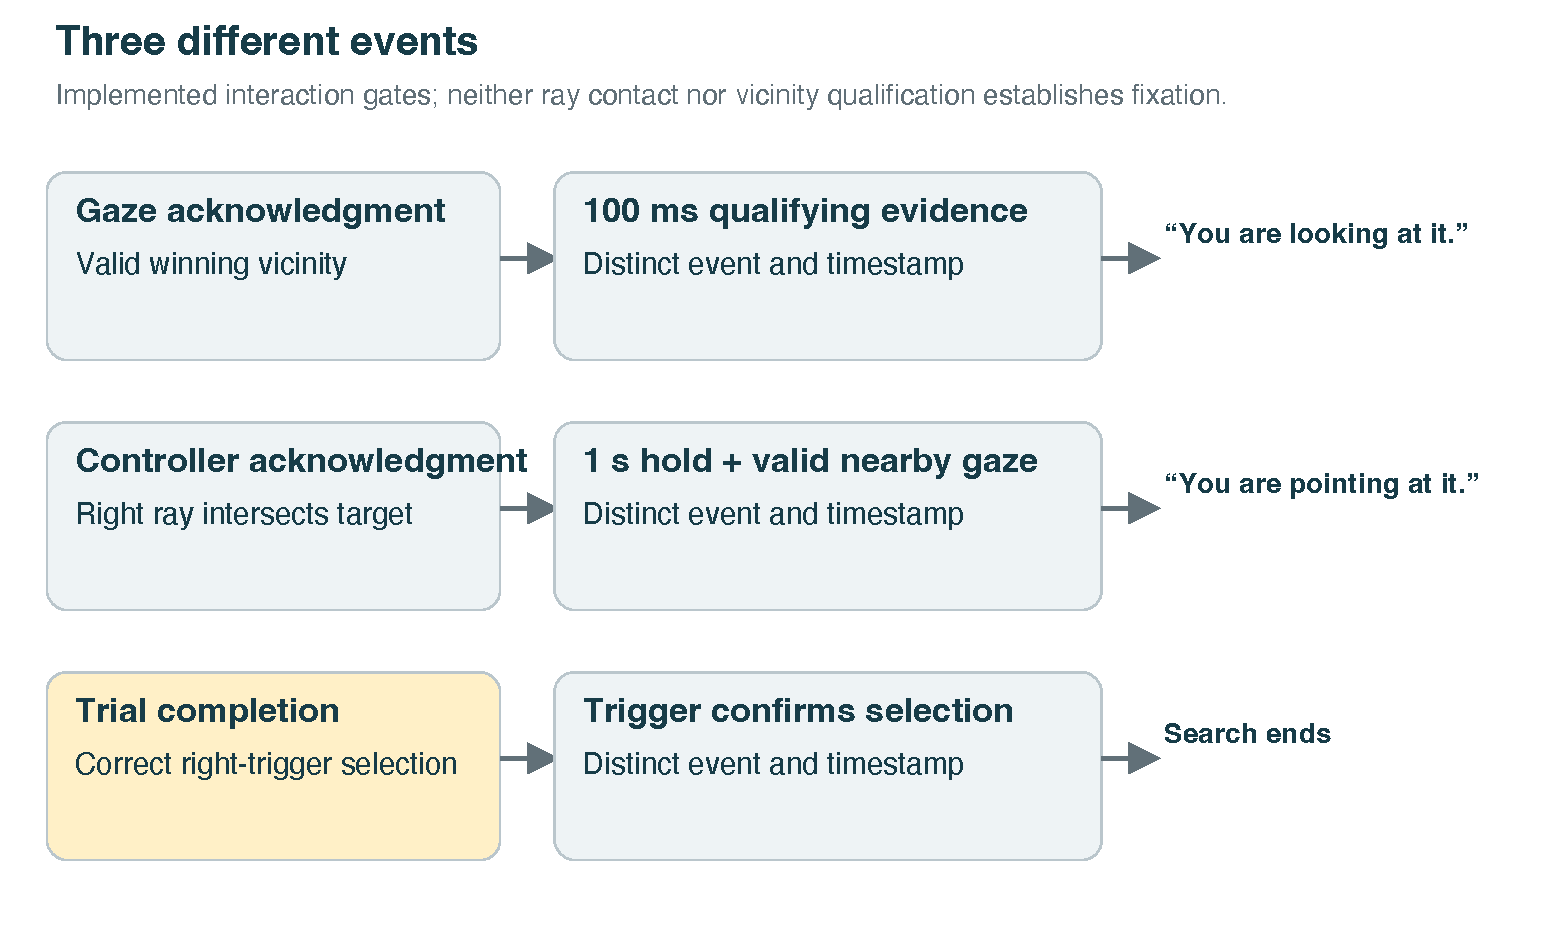
\includegraphics[width=\linewidth,alt={Three separate rows show qualified gaze, qualified controller pointing, and correct trigger selection as distinct events.}]{figures/evidence-events.pdf}
\caption[Gaze acknowledgment, pointing acknowledgment, and completion]{Implemented interaction distinctions. Gaze acknowledgment uses a 100-ms qualifying vicinity gate; pointing acknowledgment uses a one-second controller hold with required valid nearby gaze. A correct trigger selection completes the trial independently of whether either acknowledgment was spoken. These are interaction gates, not validated fixation measures.}
\label{fig:evidence-events}
\end{figure}


\subsection{Motion, Coverage, and Instructions}
Gross translation sums Euclidean differences between adjacent valid head positions, and gross rotation sums shortest quaternion angular differences. Invalid intervals, excessive gaps, and pauses break the accumulation. Gross movement is a total, not a rate. If a separate movement-rate outcome is derived, its denominator is observed covered time rather than the entire nominal session, so that runs with different data loss remain comparable.

Fixed-axis components derived from rotation vectors differ from Euler yaw, pitch, and roll and are labeled by their actual calculation. Head motion is also only an indirect measure of swivel-chair rotation, because the head can move relative to the torso and chair.

Instruction counts are based on actual software playback starts. Requested cues, rejected model answers, and prefetched clips are not counted as delivered instructions. Opening cues, search guidance, acknowledgments, reminders, and success speech have separate categories. The planned total of delivered active-search assistance includes directional guidance, gaze/pointing acknowledgments, and selection reminders. Each category is also reported separately, and opening and success speech remain outside that total. Interrupted speech counts as started speech but retains its completion status, since the participant may not have heard the full utterance.

